\chapter{Stand der Forschung und Stand der Technik}

Das Projekt ist eine pädagogische Umsetzung für Pflege Studenten im Bereich E-Learning mit aktuelle Web Technologie. Die Konzept des Projekts basiert auf die Theorien über E-Learning und VR-Training. Und die Implementierung des Porjekts profitiert von der Entwicklung der Technik Virtuelle Realität(VR), beziehungsweise im Fachbereich Web VR.

\section{Stand der Forschung}
 \subsection{E-Learning}
 E-Learning ist kein neuer Begriff, je doch ist es nicht einfach, eine epigrammatische Definition zu finden, weil E-Learning mit vielfältigen Fächern verbindet. Je nach Schwerpunkt sogar Periode fallen die jeweilligen Definitionen unterschiedlich aus.

E-Learning umfasst laut Kerres \citep{1} \glqq bei denen elektronische oder digitale Medien für die Präsentation und Distribution von Lernmaterialien und/oder Unterstützung zwischenmenschlicher Kommunikation zum Einsatz kommen.\grqq

Die Evolution der Web Technologie von \glqq Web 1.0 \grqq\ zu \glqq Web 2.0\grqq \citep{3}, nämlich von \glqq the Read Web \grqq\ zu \glqq the Read-Write Web\grqq \citep{4} bietet mehr technische Möglichkeiten für E-Learning. Stephen Downes \citep{2} zeichnet E-Learning ab 2005 als E-Learning 2.0. Da \glqq entwickelt sich E-Learning mit dem World Wide Web als Ganzes weiter und ändert sich so stark, dass ein neuer Name entseht.\grqq

In dieser Arbeit wird der Begriff E-Learning als synonym des E-Llearnings 2.0, erfahrungsgemäß Online Learning benutzt.
 
Zurzeit bezieht Internet sich auf notwendige Infrastruktur, deren Geschwindigkeit, Stabilität und Mobiliät immer verbessert werden. Der Form des Rechners ist auch unterschiedlich, Desktop, Laptop, Tabllet, Smartphone und VR Geräte. Die entwickelde Technik garantiert die stabile und vielfältige Nutzung von E-Learning. Im Jahr 2013 haben 35\% der Deutschen E-Learning-Erfahrung.

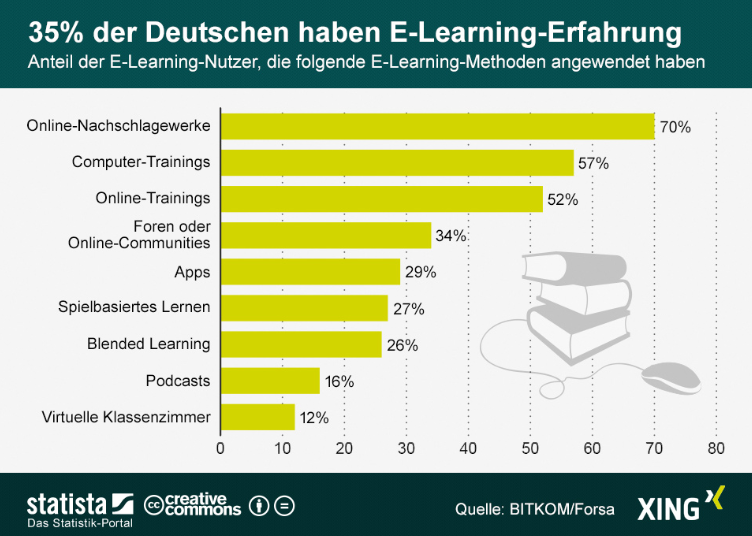
\includegraphics[width=\textwidth]{images/eLearningErfahrung.png}

Nach der veröffentliche Statistik ist die prognostische Umsätze durch E-Learning weltweit von 2016 bis 2021 mehr als 30.000 millionen US-Dollar jedes Jahr.

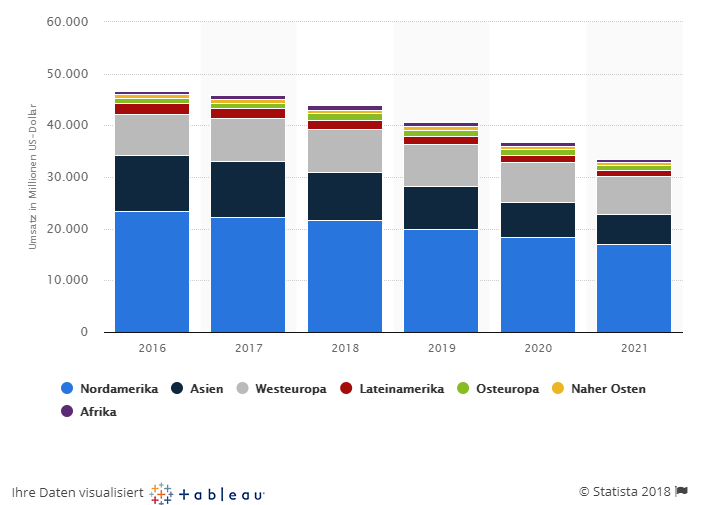
\includegraphics[width=\textwidth]{images/umsatzDiagnose.png}

E-Learning ist schon ein unverzichtbares pädagogisches Mittel und hochwertiger wirtschaftliche Markt. Und auf dem E-Learning Markt spielt die Hochschulen eine überwiegende Rolle.

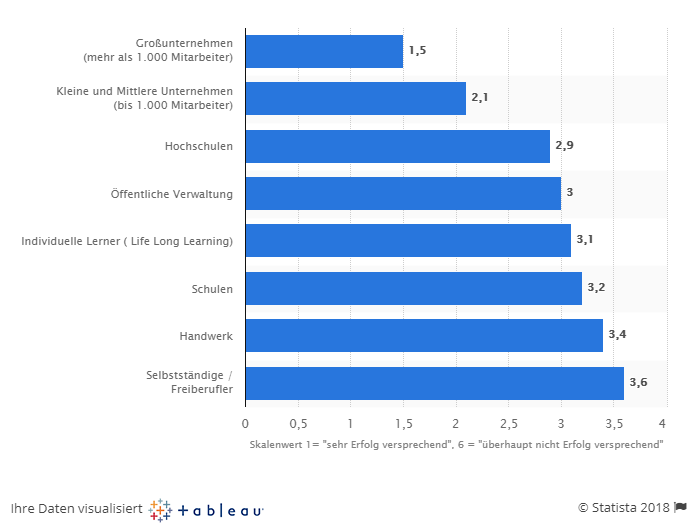
\includegraphics[width=\textwidth]{images/zielgruppe.png}

Als ein wichtiges Werkzeug im Bereich Ausbildung sind sieben Merkmale des E-Learnings Laut Justin Ferriman \citep{6} eindeutig:

\begin{enumerate}
\item Skalierbar: Inhaltliche Änderung ist flink. 
\item Kapazität und Konsistenz: Pädagogen können eine große Reichweite für ihre Zielgruppe erreichen und die Botschaft wird auf konsistente Weise kommuniziert.
\item Hohe Aufbewahrung: Vielfältige Learning-Ansätze führen zu höher Aufbewahrung.
\item Zeitliche und finanzielle Ersparnisse: E-Learning entfernt die Bedürfnisse der Reise und Stelle.
\item Aktivitäts- und ROI(Return On Investment)-Messungen: Der Erfassen des Lernfortschritts und die Berichterstellung der Lernaktivitäten sind mühelos und anschaulich.
\item Reduzierung von CO2-Fußabdruck: Wenige Reise und Ausdruck reduziert der Kohlendioxid-Ausstoß.
\item Flexibel: Es gibt keine zeitliche oder geografisch Begrenzung für die Studenten.
\end{enumerate}\

Um bessere E-Learning Projekt zu entwickeln, sollen die Nachteilen des E-Llearnings erkannt werden. Im Jahr 2011 hat Ao.Univ.-Prof.Dr. Karl Leidlmair\citep{7} elf Nachteile von E-Learing gelistet. Obwohl nach sieben Jahren im Jahr 2018 einige Mängel z.B. \glqq Das Angebot an Qualitätsprodukten am Markt ist Überschaubar \grqq\ nicht sehr angepasst sind, sind viele Auffassungen nach wie vor sinnreich.

\begin{enumerate}
\item Technische Abhängigkeit: Rechner und Internet sind die Grundlage des E-Learnings, und mehr neu Technik werden zu Verfügung stehen, z.B. VR und AR(augmented reality).
\item Kein Sozialer Kontakt: Obwohl Chat-Rooms, video conferencing sogar VR meeting werden in E-Learning eingesetzt, ist der direkte menschliche Kontakt nicht ersetzbar.
\item Mangelnde praktische Teile: Die praktische Übungen im Labor sind besonders schwer mit E-Learning durchzuführen.
\item Disziplin und Selbstlernkompetenz: Die Motivation und die Kontinuität können nicht garantieren.
\end{enumerate}\

Noch ein nachteiliger Punkt, den von Richard Nolan\citep{5} genannt, kann als eine Ergänzung für die Ansicht von Prof. Dr. Karl Leidlmair gelten. Die Feedbacks könnten nicht genug und rechtzeitig. Aufgrund der zeitlichen Freiheit des E-Learnings können die Studenten jederzeit lernen, außerdem können die Zahl der Lernenden sehr umfangreich sein, deswegen werden die rechtzeitige Feebacks, besonders die Antwort der individuellen Fragen sichergestellt.

Das E-Learning ist schon weitläufig benutzt und Aufmerksamkeit geschenkt, aber ist es echt effekitver und effizienter als traditionelle pädagogische Mittel, die im Klassenzimmer gemacht werden? Um die Frage zu antworten, hat Will Thalheimer\citep{8} eine Metaanalyse durchgeführt. Die Lernmethoden, beispielsweise Karteikarten, Brainstorming und Tests, gelten als Einflussfaktoren im Vergleich zwischen die Modalitäten des Lernens, nämlich E-Learning und der Unterricht im Klassenzimmer. Aus der Untersuchung mit 28 Arbeiten ergibt sich die Folgerung:

\begin{enumerate}
\item Wenn die Lernmethoden gleichbleibend sind, produzieren beide das gleiche Ergebnis.
\item Wenn die Lernmethoden nicht gleich sind, E-Learning übertrifft die Unterricht im Klassenzimmer.
\item Der Effekt von E-Learning kann besser, schlimmer, manchmal auch gleich wie der Effekt des Unterrichts im Klassenzimmer sein.
\item Die Modalitäten des Lernens spielen keine wichtige Roller für die Lerneffektivität, sondern die Lernmethoden wie realistische Praxis, beabstandete Wiederholung, realer Kontext und Feedback.
\item Die Mischung mit E-Learning und die Untericht im Klassenzimmer hat die beste Wirkung. Wahrscheinlich ist der Grund, dass mehr effektive Lernmethoden eingesetzt werden können. 
\end{enumerate}\

Zusammenfassung der Forschung kann sein, dass der größte Vorteil des E-Learnings ist, mehr effektive Lernmethoden anzubieten.

Dank für die schnell entwickelnde Web Technik werden mehr Lernmethoden ermöglicht. In dem Bericht \glqq Elearning market trends and forecast 2017 -2021\grqq\ von Docebo werden die fünf wichtigste Technologien ausgelistet, die mit E-Learning integriert werden. Die Anwendung der Technologien werden die Effektivität und die Effizienz des E-Learnings verbessern.

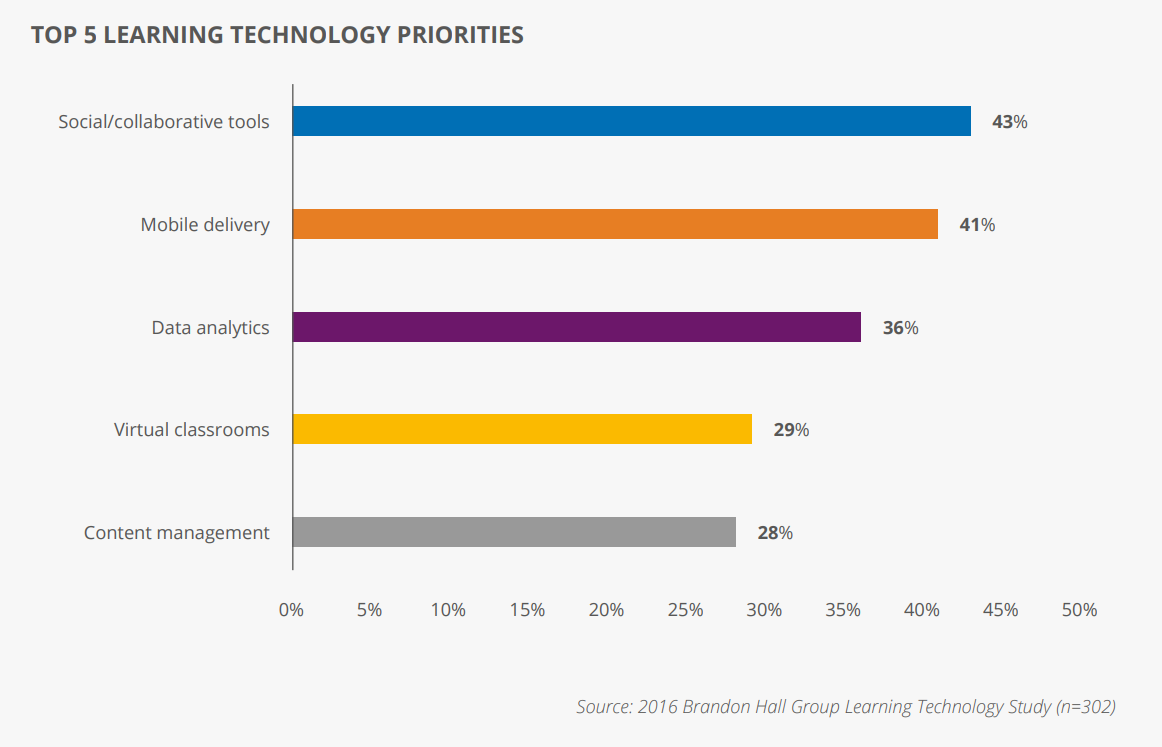
\includegraphics[width=\textwidth]{elearningtop5technology}

Fast ein Drittel der gefragten Unternehmen finden, dass virtueller Klassenraum eines hilfreiche Werkzeug für die Schulung wird.

 \subsection{VR-Training}
 
Virtuell Realität(VR) ist die Technik, die die Situation \glqq Interaktiv erzeugte multimodale Sinneseindrücke 2. Ordnung, die von Menschen als solche 1. Ordnung wahrgenommen werden.\grqq\ \citep{9} realisiert. Kurzbeschreibung: Mit VR Technik wird der Benutzer in einer virtuellen Umgebung eingebracht.

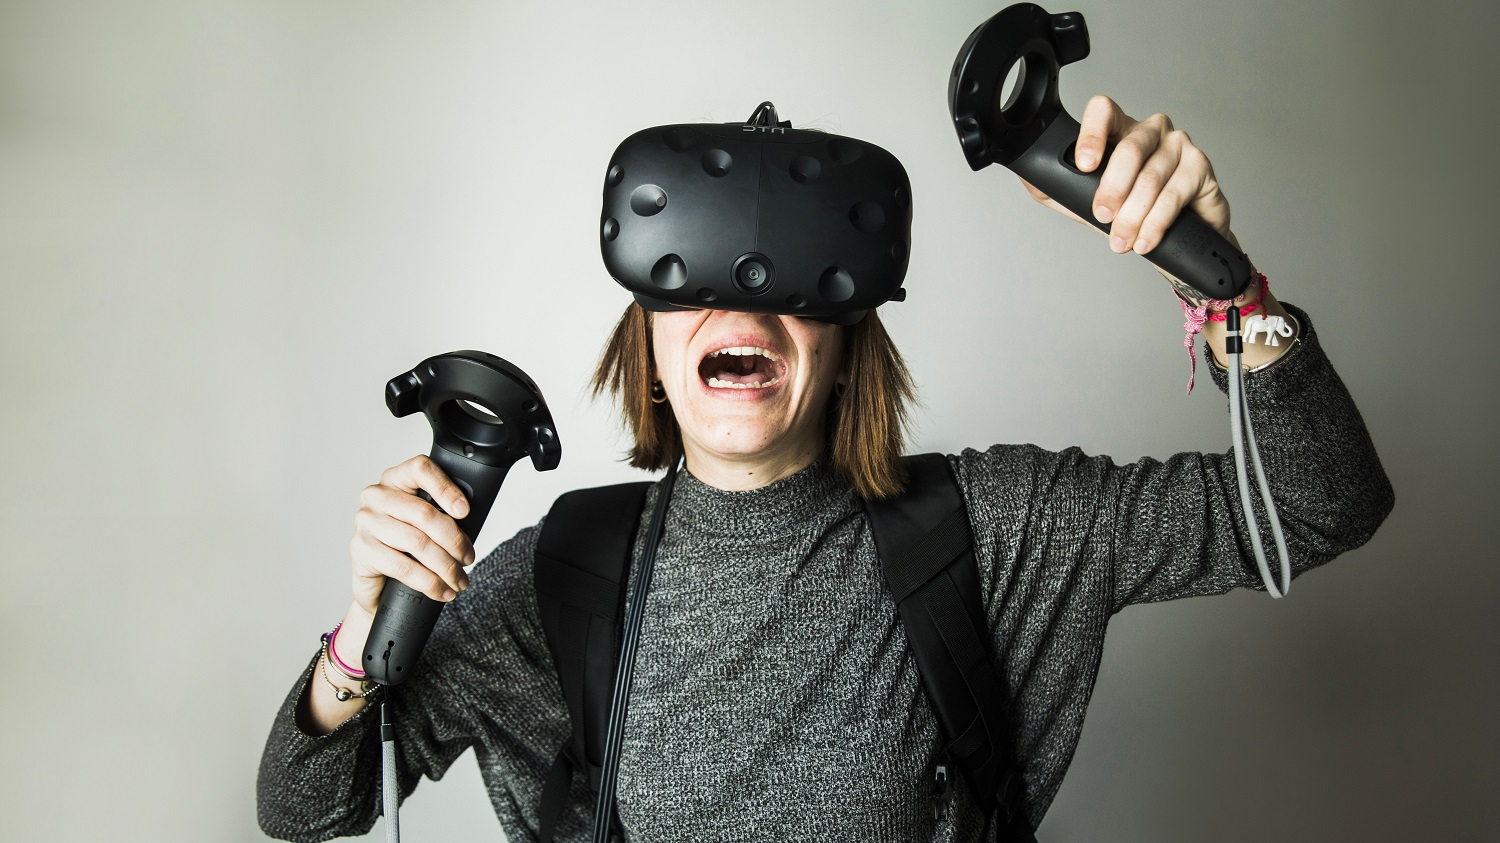
\includegraphics[width=\textwidth]{images/vrhtcvive.jpg}

VR-Training ist das Synonym von virtual reality-based training (VRBT). \glqq VRBT ist eine interaktive und umfassende Unterrichtsmethode, bei der mithilfe von Technologien virtuelle Szenarien bereitgestellt werden, um Situationen zu simulieren, die in tatsächlichen Umgebungen auftreten können. \grqq\ \citep{14}

Das immersive Erleben entscheidet sich, dass die VR Technik geeignet für Training ist.

Laut der Forschung von James Clark und Allan Paivio\citep{10} wird die Gedächtnisleistung verstärkt, wenn multisensorische und emotionale Wahrnehmungen eingegeben werden. Die Forschung von S.A. Christianson\citep{11} stimmt überein, dass je stärker eine emotionale Reaktion auf einen Reiz ist, desto stärker wird das Gedächtnis sein. 

\glqq VR ist ein wirksames Medium zur Stimmungsinduktion, das seinen Einsatz in verschiedenen Anwendungsbereichen eröffnet, die von der Wohlbefinden-Branche bis zur klinischen Psychologie reichen. \grqq\ \citep{29} Was noch wichtig ist, dass die simulierte Szenario wiederholbar und die dargestellte emotionale und stressige Situation kontrollierbar ist, deswegen wird VR eine wichtige Rolle im Bereich neurowissenschaftlichen Forschung und Therapie spielen.\citep{13} Laut der Forschung von Albert A. Rizzo kann VR Technik als Hilfsmittel bei der Behandlung für Phobien benutzt werden.\citep{12}

Eine Studie\citep{30} beweist die Förderung der VR Technik für Gedächtnisleistung. Die Probanden werden in 2 Gruppe geteilt. Eine Gruppe schaut ein 2D Video an. Die andre Gruppe schaut ein 360\degree\ Video, deren Inhalt gleich wie die 2D Video ist, mit VR Breille. Nach 48 Stunden kann die VR Gruppe besser an der Inhalte des Videos als 2D Gruppe erinnern.

Im Buch \glqq The VR Book: Human-Centered Design for Virtual Reality \grqq wird die Immersion in sechs Kategroien eingeteilt: \citep{28}

\begin{enumerate}
\item \textbf{Extensiveness} beschreibt die Stärke und Menge der aufgerufene Wahrnehmungen (z.B optische, akustische).
\item \textbf{Matching} erfasst die Anpassung der Feedback in virtuelle Umgebung für die Interaktion (z.B Kopfbewegungen).
\item \textbf{Surroundness} ist die räumliche Repräsentation (z.B Blickfeld, räumlicher Sound).
\item \textbf{Vividness} erfasst die technische Implementierung für eine lebendige Simulation (z.B Auflösung, Material)
\item \textbf{Interactablility} beschreibt die Möglichkeiten der Interaktion, um die Objekten in virtuelle Umgebung zu beeinflussen (z.B clicken, drücken)
\item \textbf{Plot} beschreibt das Verhalten, die nach dem Regel der realen Wert in virtuelle Umgebung gemacht werden.
\end{enumerate}\

Durch die Studie von Doug A. Bowman wird es gefunden, dass die lebendiger Immersion zu besserem räumlichen Verständnis und höherer Leitung für interaktive Aufgaben führen kann. \citep{27}


Als neue technische Anwendung im Bereich Schulung hat VR-Training überragend Vorteile\citep{15}:

\begin{enumerate}
\item VR macht schulung visueller: Die immersive Darstellung der 3D Szenario mit VR ist visueller und attraktive als 2D Darstellung wie Videos, Bilders und Text.
\item VR macht Schulung sicherer: In viele Arbeitsbereich wie Fertigung, Energie und Verteidigung ist die Unfälle während der Schulung schwer zu vermeiden. Mit Hilfe der VR Technik können die Praxen in simuliert Umgebung durchgeführt werden, die Risiko der Unfälle fernzuhalten.
\item VR macht Schulung erschwinglicher: Die Kosten für Schulung können sehr teuer sein, besonders wenn die Materialien nicht wiederverwendbar sind. Außer der Ausgabe von VR Geräte und Entwicklung kostet VR-Training wenig Geld.
\item VR macht mehr Fernschulung möglich: Durch VR Technik können vielen Praxen entfernt durchgeführt werden.
\item VR macht Aufbewahrung und Rückruf der Schulung möglich: Durch VR Technik kann der Durchlauf gespeichert werden, Und eine bestimmte Aktivität mehrere Male üben.
\end{enumerate}\

Die Auffassung von SIMBLOG\citep{16} ergänzt die Vorteile:

\begin{enumerate}
\item Komplexe Probleme und Situationen vereinfachen: Mit VR Technik kann die komplexe Situation als kleine Teile geteilt.
\item Mehr Spaß machen: Mit VR Technik können die Übungen \glqq gamable \grqq\ sein, um der Benutzer zu motivieren. 
\end{enumerate}\

Noch ein bedeutsamer Vorteil ist, dass VR-Training das Schulungsproject durch die gesammelte Daten während der Übung verbessern kann. \glqq Oft ist es schwierig oder unmöglich, die Leistung zu verbessern, ohne die zugrunde liegenden kognitiven Faktoren zu kennen, die die Leistung beeinflussen. Die einzigartige, von STRIVR entwickelte VR-Aufmerksamkeitsanalyse ermöglicht diesen Einblick. \grqq\ \citep{18}
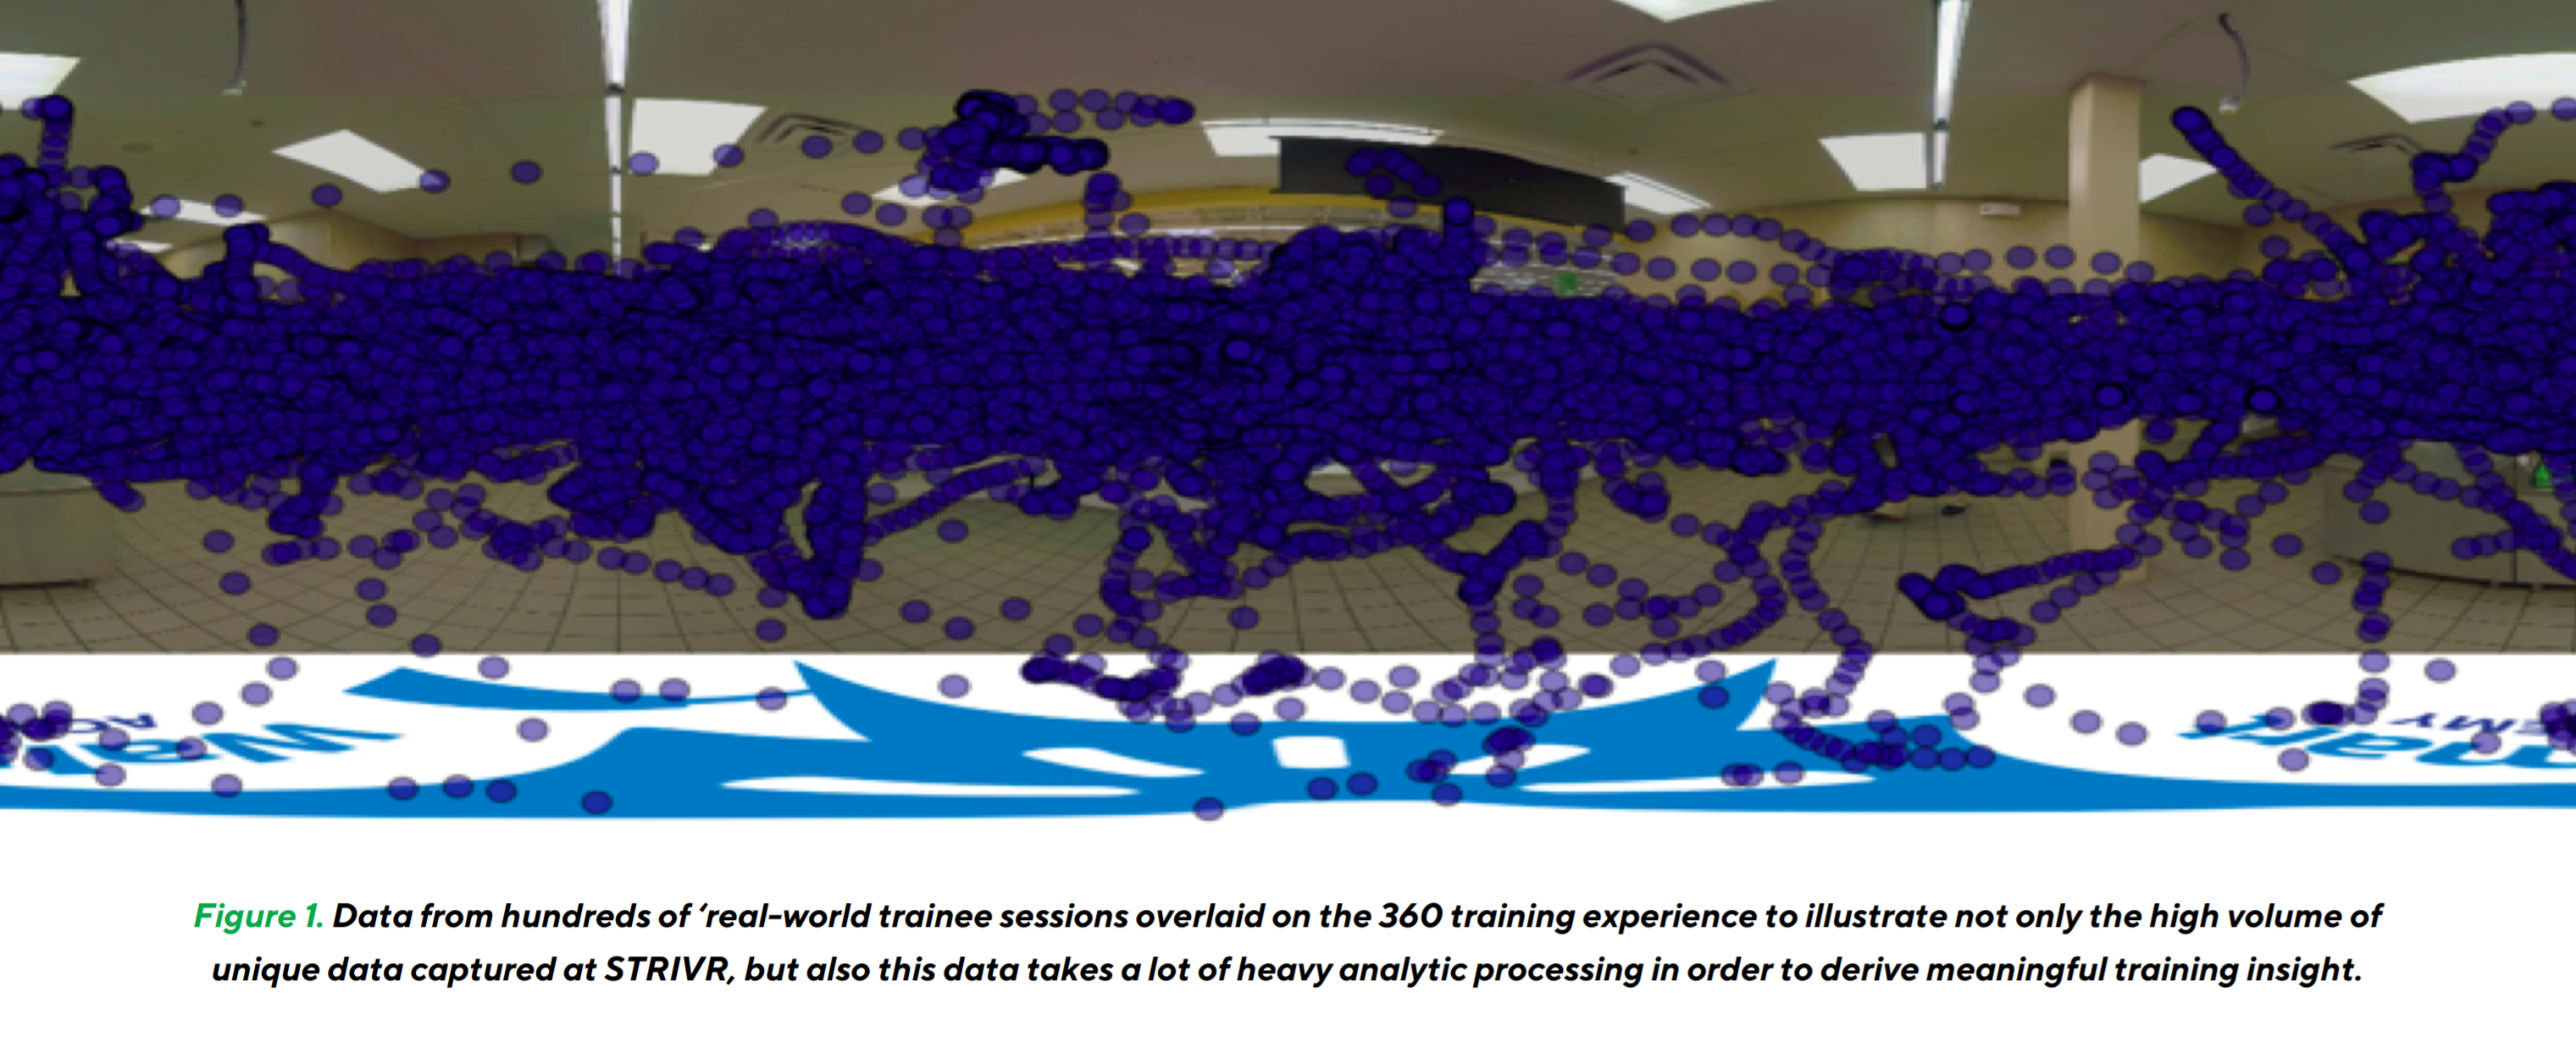
\includegraphics[width=\textwidth]{images/intentionanalys1.png}
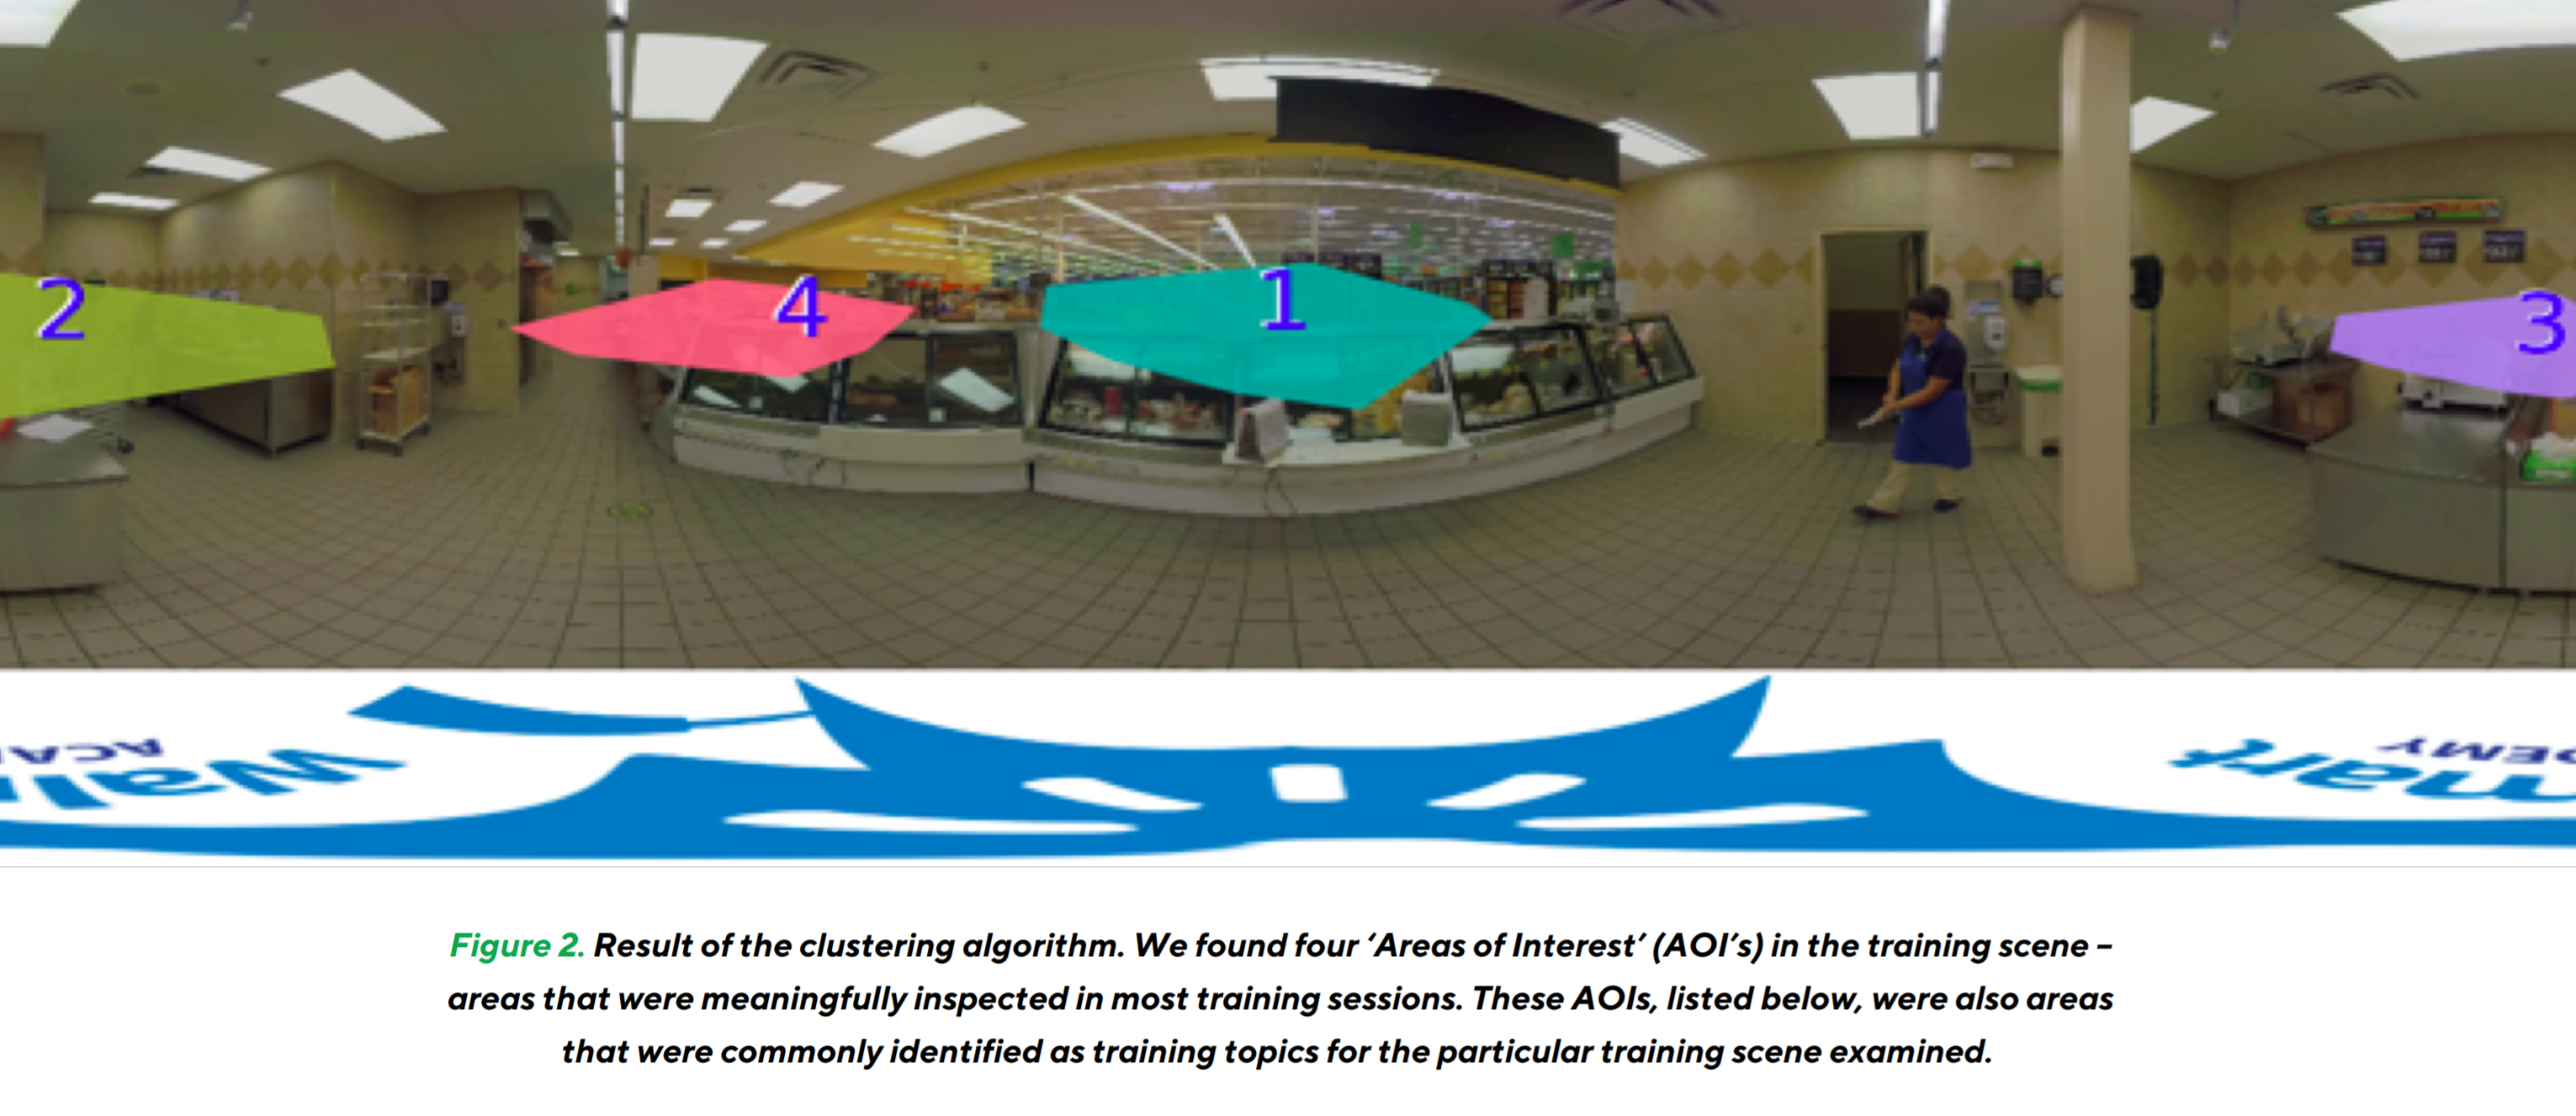
\includegraphics[width=\textwidth]{images/intentionanalys2.png}

Die Nachteile sollen nicht ignoriert werden\citep{17}:

\begin{enumerate}
\item Beeinträchtigt die menschlichen Verbindungen: VR-Training könnte die Notwendigkeit der menschlichen Kommunikation reduzieren.
\item Mangel an Flexibilität: Menschliche Kommunikation ist flexibel. VR-Training kann nicht für alle mögliche Aktivitäten Feedback geben.
\item Funktionsprobleme: Jede Software könnte Bugs haben. Das VR-Training könnte die Schulung wegen Bugs behindern.
\item Ziemlich teuer: Obwohl Google Cupboard eine günstige Möglichkeit anbieten, kann nicht jede Smartphone den Aufwand des VR Programms leisten. Für PC ist die Anforderung der Leistung noch stärker.
\end{enumerate}\

\section{Stand der Technik}
 \subsection{Virtuelle Realität(VR)}
  \subsubsection{Technologie}
Carolina Cruz-Neira hat die technologieorientierte Definition von VR gegeben \glqq Virtual Reality refers to immersive, interactive, multi-sensory, viewer-centered, three-dimensional computer generated environments and the combination of technologies required to build these environments.\grqq\ \citep{19}
  
Die Implementierung der VR Technik liegt an der menschlichen Tiefenwahrnehmung, die auf der Fähigkeit zu \glqq stereoskopischem Sehen \grqq\ beruht.\citep{20} Die Augen übertragen die Bilder, die auf Netzhaut gebildet werden, zum Gehirn. Durch die Analyse auf die überlappte Teile der Bilder von links und rechts Augen wird die Tiefenwahrnehmung erstellt, dadurch man die Objekten in 3D sehen kann.

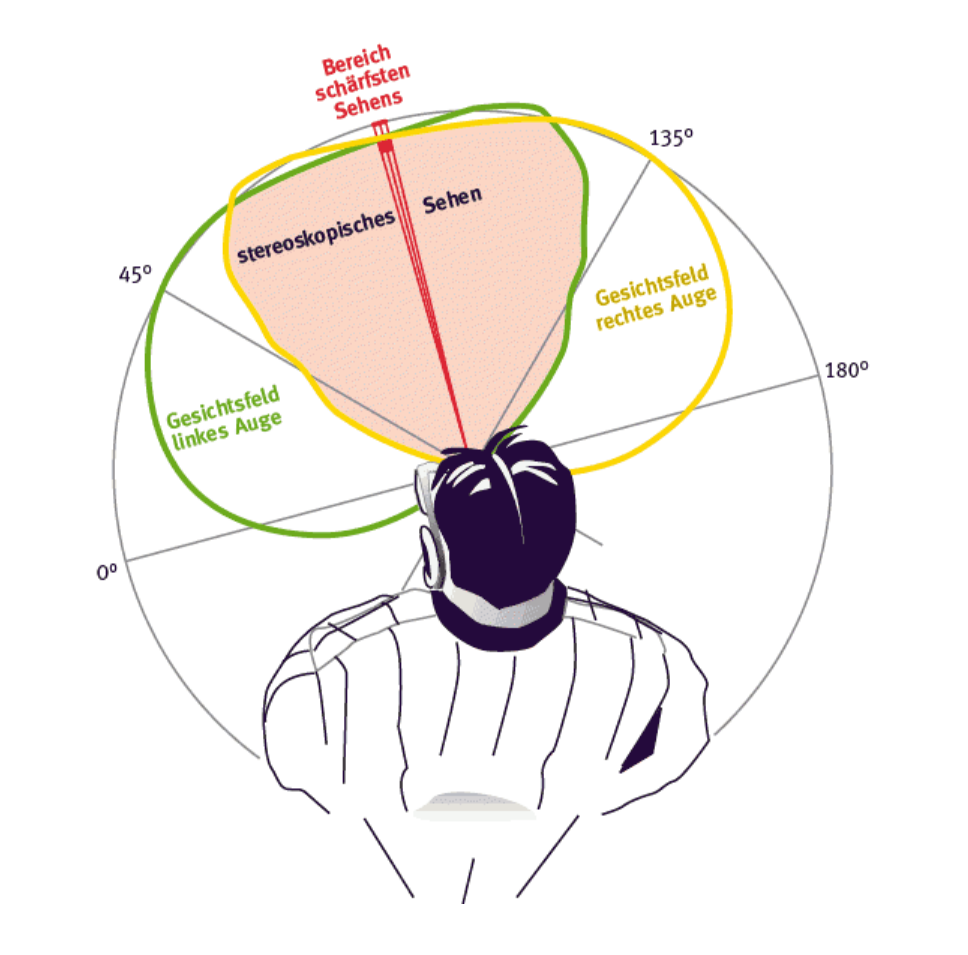
\includegraphics[width=\textwidth]{images/stereoskopischesSehen.png}

In HMD (Head mounted display) von VR werden die angepasste Bilder für links und rechts Augen getrennt kurz vor der Augen dargestellt. Die Bilder werden im Gehirn gerechnet, um räumliche Wahrnehmung aufzubauen. Sodass wird die Szenario, die in HMD gezeigt wird, als 3D Umgebung von dem Benutzer gesehen.

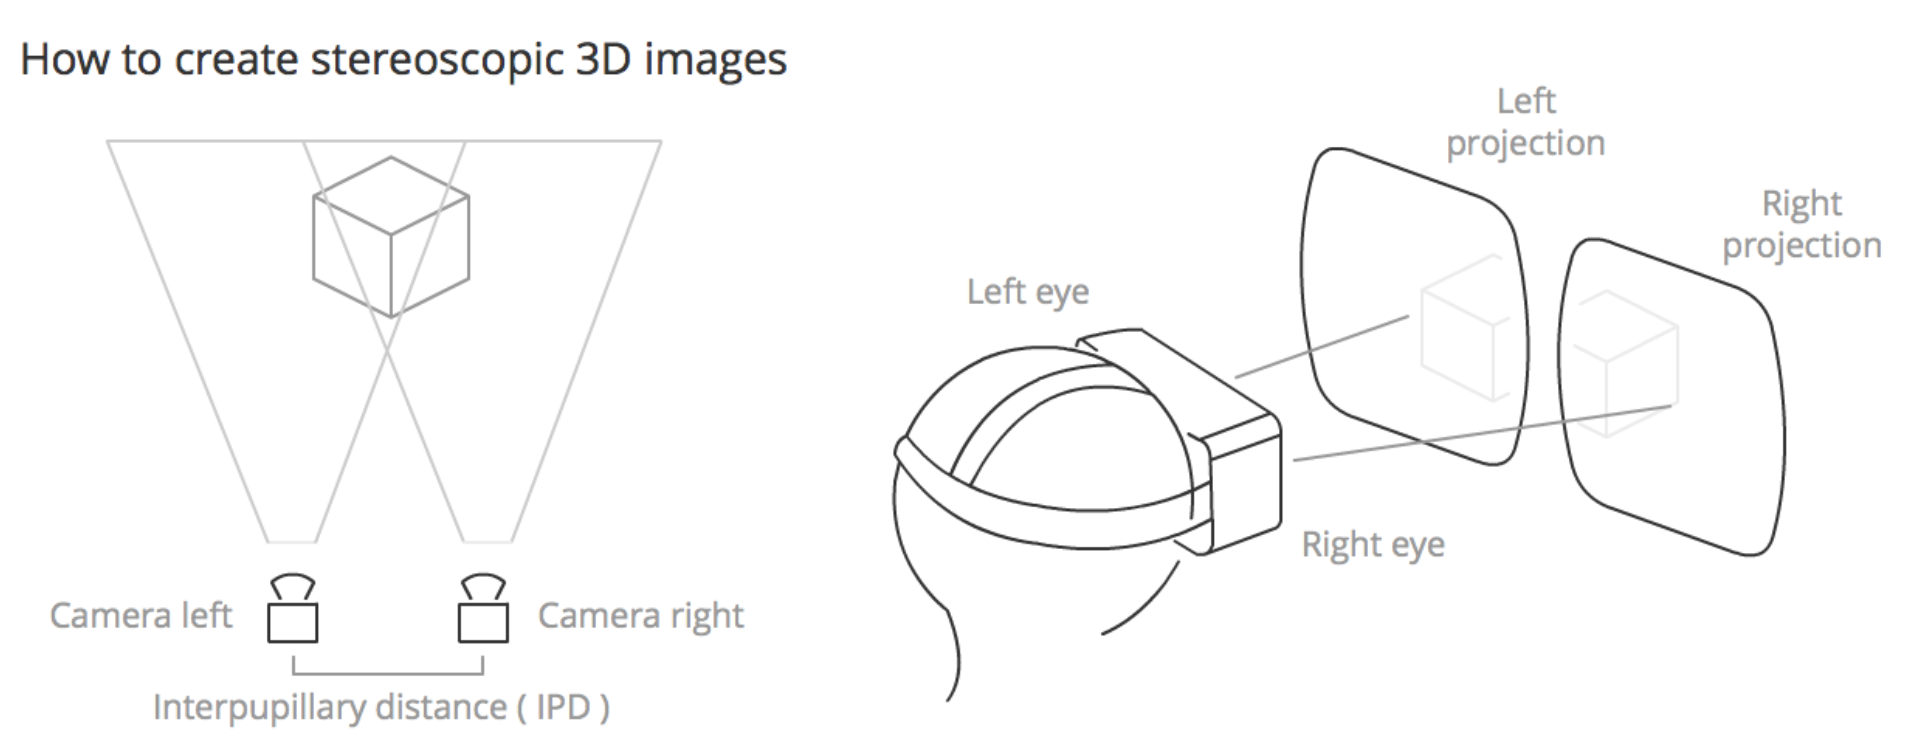
\includegraphics[width=\textwidth]{images/howToCreate.png}

  \subsubsection{Geräten}
  Typische VR Geräte bestehen aus drei Teilen, nämlich HMD, Rechner und Controller. HMD ist der Hauptteil der VR Geräte. Und es gibt unterschiedliche Typen für HMD.
  
  Nach dem Form des Rechners können HMDs in zwei Gruppen klassifiziert werden können: unmobile und mobile.
  
  Unmobile HMD bedeutet, dass der Rechner(Desktop oder Leptop) nicht in HMD eingepackt werden kann. Meistens verbindet der Rechner durch einem Kabel mit dem HMD, z.B. Oculus Rift und HTC Vive. Die Vorteile davon sind, dass die Leistung stark ist, die Kapazität der Speicher groß ist und die Wärmeableitung kräftig ist. Die Nachteile sind, dass die Kosten hoch ist, weil einen extra Rechner notwendig ist. Und die Netzteile für Rechner und HMD sind gefordert, deshalb ist die Bewegung während der Nutzung begrenzt.
  
  Mobile HMD bedeutet, dass der Rechner in HMD eingepackt kann oder in HMD integriert ist. Der eingepackte Rechner ist normalerweise Smartphone. Die Beispiele davon sind Google Cupboard, Gear VR, Daydream Vr. Die andere Variante ist, dass der Rechner integriert wird, deswegen ist ein extra Smartphone unnötig, z.B. Oculus Go und Lenovo Mirage Solo. Die Vorteile der mobile HMDs sind, dass die Größe der Geräte klein ist, der Netzteil während des Anwendens nicht gebraucht ist, der Preis ziemlich niedrig ist. Die Nachteile sind, dass die Leistung relativ schwach und die Kühlung kraftlos ist.
  
  Nach der Möglichkeiten der Bewegung können die HMD in zwei Gruppe unterteilt werden, 3 DoF (Tree degree of freedom) und 6 DoF (Six degree of freedom).
  
  Degree of freedom beschreibt die Bewegung eines Objekts in einem Raum. Es könnte als \glqq verschiedene grundlegende Möglichkeiten, wie sich ein Objekt bewegen kann \grqq erklärt \citep{25}. Es gibt insgesamt 6 DoF, und sie können tatsächlich in 2 verschiedene Typen unterteilt werden: Translationen und Rotationen.
  
  Translation bedeutet räumliche Bewegung in einem Raum. Das Objekt kann auf drei Achsen bewegen. Die drei Achsen gelten als \glqq three degree of freedom\grqq .
  
  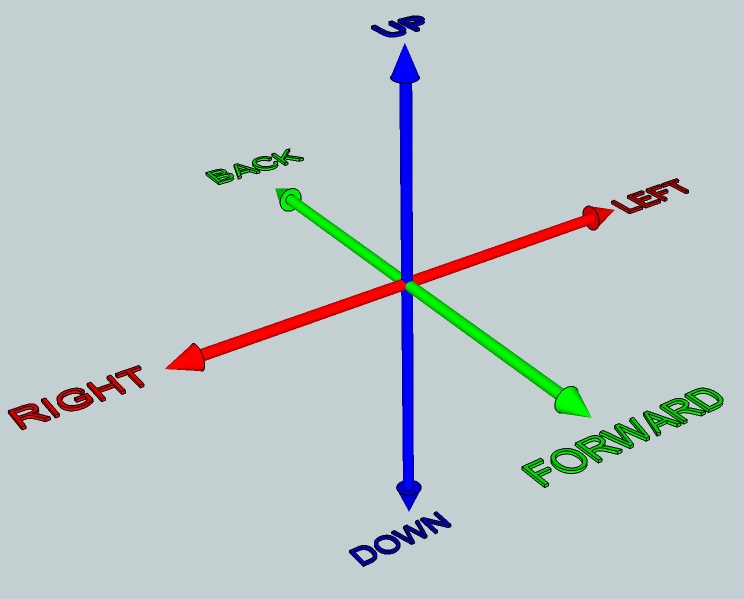
\includegraphics[width=\textwidth]{images/translations-diagram.jpg}
  
  Rotationen bedeutet kreisförmige Drehung. Das Objekt kann auch auf drei Achsen drehen, die als andere \glqq three degree of freedom\grqq gelten.
  
  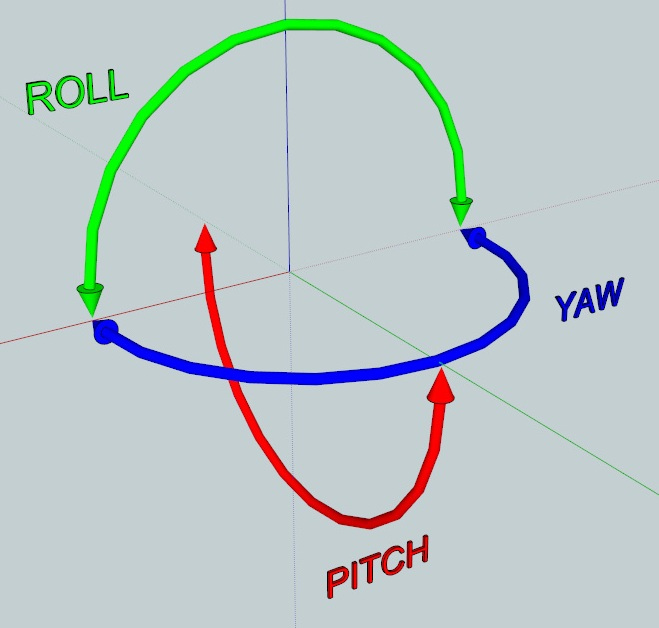
\includegraphics[width=\textwidth]{images/rotations-diagram.jpg}
  
  Wenn ein HMD 3DoF ist, kann es normalerweise nur die Rotationen erkennen. Wegen der Begrenzung der Leistung ist erfahrungsmäßig mobile HMD 3DoF HMD.
  
  Im Vergleich zu 3Dof HMD kann 6Dof HMD nicht nur die Rotationen sondern auch die Translationen erkennen. Durch externem starken Rechner kann die unmobile HMD die Aufwendig Rechnen leisten.
  
   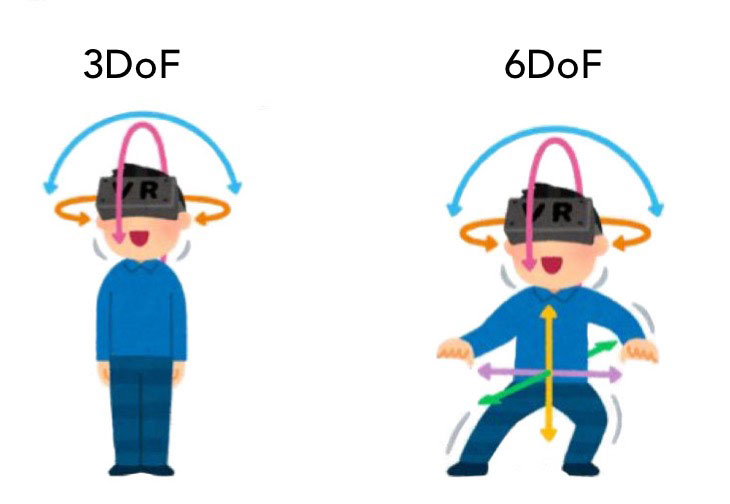
\includegraphics[width=\textwidth]{images/6DoF-vs-3DoF.jpg}
  
  Theoretisch wird 3Dof Controller z.B. Gear VR Controller und Daydream VR Controller für 3Dof HMD ausgestattet. Die Position von 3DoF Controller in dem Raum ist fest. Die Interaktion zwischen die Objekten und dem Controller wird durch einem von Controller strahlenden Raycaster aufgerufen.

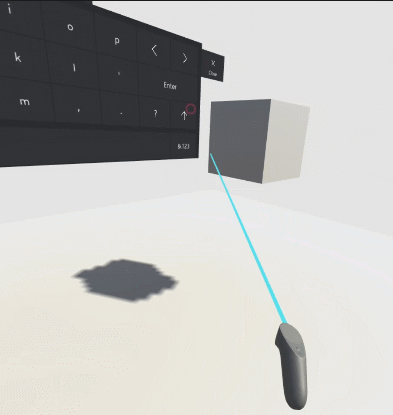
\includegraphics[width=\textwidth]{images/3dcontroller.png}
  
  Es gibt auch HMD wie Google Cupboard und alte Gear VR, die kein Controller haben. Normalerweise steht ein Knopf oder ein Trackpad an der Seite des HMDs für Interaktion zu Verfügung.
  
  6DoF Controller werden mit 6Dof HMD zusammen benutzt. Es bietet größte interaktive Freiheit in einem Raum. 
  
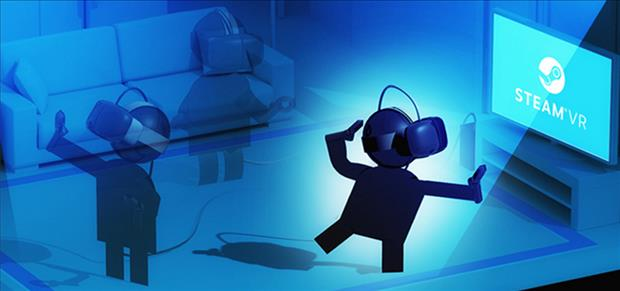
\includegraphics[width=\textwidth]{images/6dcontroller.jpg}

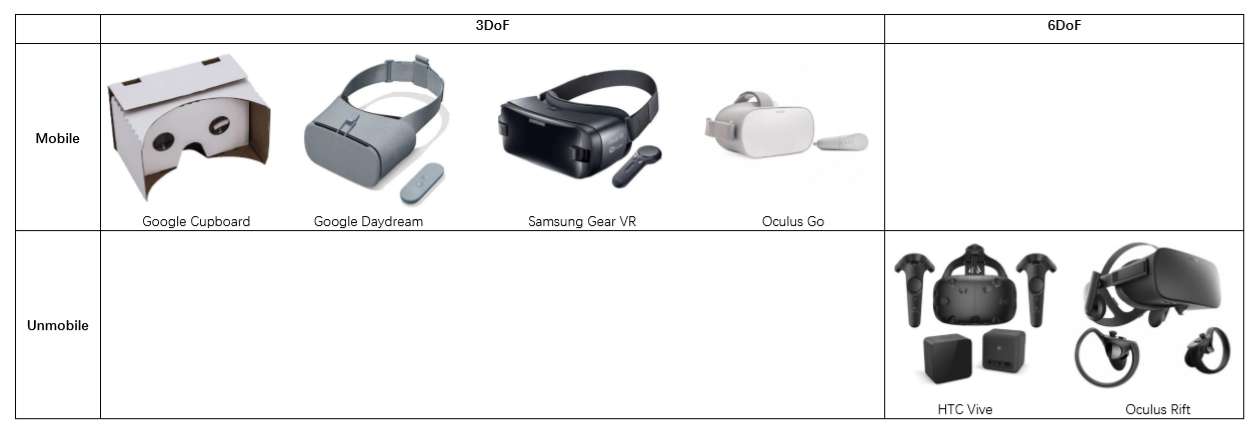
\includegraphics[width=\textwidth]{images/vrDevicesTable.png}
  
  \subsubsection{Entwicklung}
  Obwohl Unity und Unreal Engine ursprünglich Game Engines sind, spielen die beide wichtige Rollen im Bereich VR Entwicklung. Mit den Engines können VR Projekt einfach erstellen, entwickeln, debuggen und bilden. Bei der Erstellung wird die Grundstruktur des Projekts aufgebaut. Während der Entwicklung ist viele vorhandenen Funktionen wie Kollisionserkennung und Physik-Simulation zu Verfügung. Die standert IDE(Integrated Development Environment) ist Visual Studio von Microsoft. Aber ist es möglich, andere IDE zu benutzen. Wegen der engen Verbindung zwischen Visual Studio und die beiden Engines ist Debuggen durch \glqq Checkpoint \grqq\ und \glqq Breakpoint \grqq\ mühelos. Mit Game Engines können Projekte als anpassende Formate für unterschiedliche Geräte bildet werden.

  C\# ist die bevorzugte Programmirungssprache für Unity, die von Microsoft entwickelt. Eine andre Möglichkeit ist Unity Script, eine Variante von JavaScript, die freundlicher als C\# für Anfänger ist.
  
  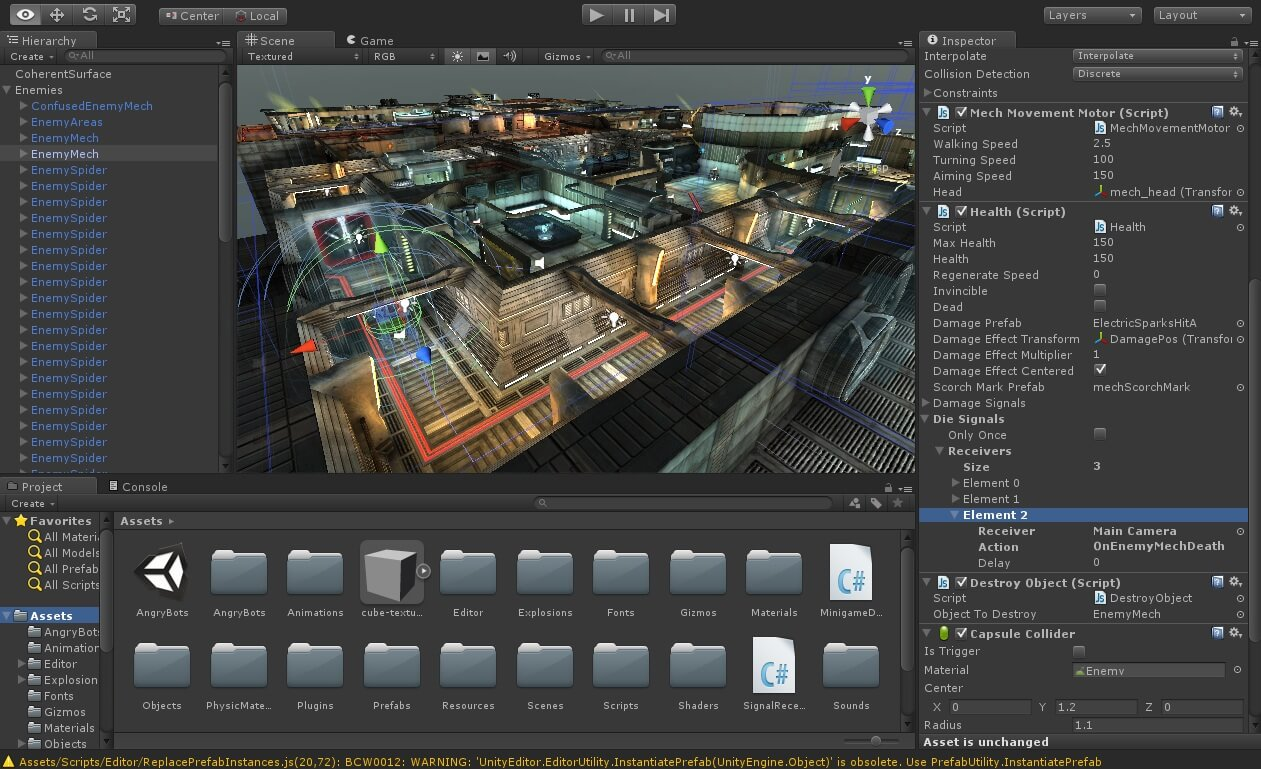
\includegraphics[width=\textwidth]{images/unity.jpg}
  
  C++ ist die standert Programmierungssprache für Unreal Engine. Außerdem wird Blueprints Visual Scripting unterstützt. Das ist eine grafische knotenbasierte Schnittstelle, um die Interaktion eines Objekts zu definieren. Die Option macht es möglich, dass die Entwicklern ohne Kenntnisse der Programmierung das Script in Unreal Engine schreiben.
  
  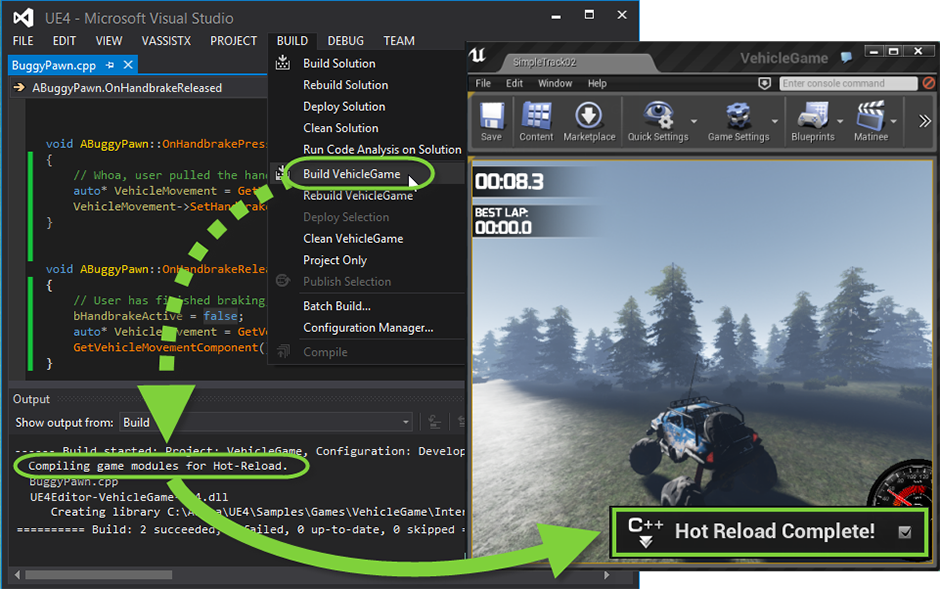
\includegraphics[width=\textwidth]{images/uec.png}
  
  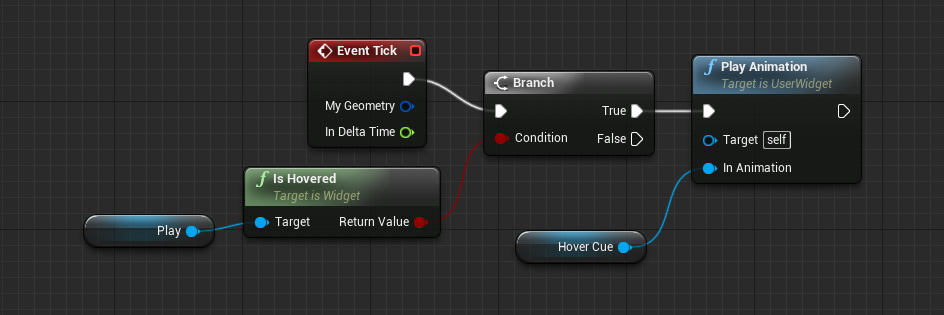
\includegraphics[width=\textwidth]{images/ueblueprint.png}
  
 \subsection{Web VR}
 Um \glqq WebVR \grqq\ besser zu verstehen, werden zwei relevante Begriffe erklärt, native Applikation(native App) und web Applikation(Web App).
 
 Native Apps werden speziell für ein Betriebssystem, z.B. IOS, Android, Macintosh und Windows programmiert und laufen dann ausschließlich auf entsprechende Geräte. Der Vorteil ist, \glqq dass alle Schnittstellen zu Hardware einheitlich funktionieren und die Ressourcen des Geräts optimal genutzt werden\grqq.\citep{22} Die Nachteile sind, dass der Aufwand der Entwicklung hoch ist, weil für jede Betriebssystem eine bestimmte Version entwickelt werden muss. Außerdem muss die native App vor dem Anwendung heruntergeladen und installiert.
 
 Web Apps werden für Browser entwickelt. Das heißt, dass sie auf Browser laufen und unabhängig von Betriebssystem sind. Der Vorteil ist die gut Erreichbarkeit. Der Aufruf ist durch der Angabe eines URLs in Browser, und Herunterladen und Installation sind unnötig. Die Nachteile sind stärke Abhängigkeit von Internet und schwächer Leistung als native Apps.
 
  \subsubsection{Technologie}
 WebVR ist ein Form von Web App. \glqq WebVR is an open specification that makes it possible to experience VR in your browser. The goal is to make it easier for everyone to get into VR experiences, no matter what device you have. \grqq \citep{21} Eines wichtige Merkmal ist, dass die Szenarien nicht nur als VR Form in HMD, sondern auch als 3D Form über den normalen flachen Bildschirm dargestellt werden können, wenn keine VR Geräte zur Verfügung ist.
 
 Obwohl zur Zeit WebVR noch nicht von allen Browsers unterstützt wird, hat WebVR ziemlich breite Zugänglichkeit.
 
 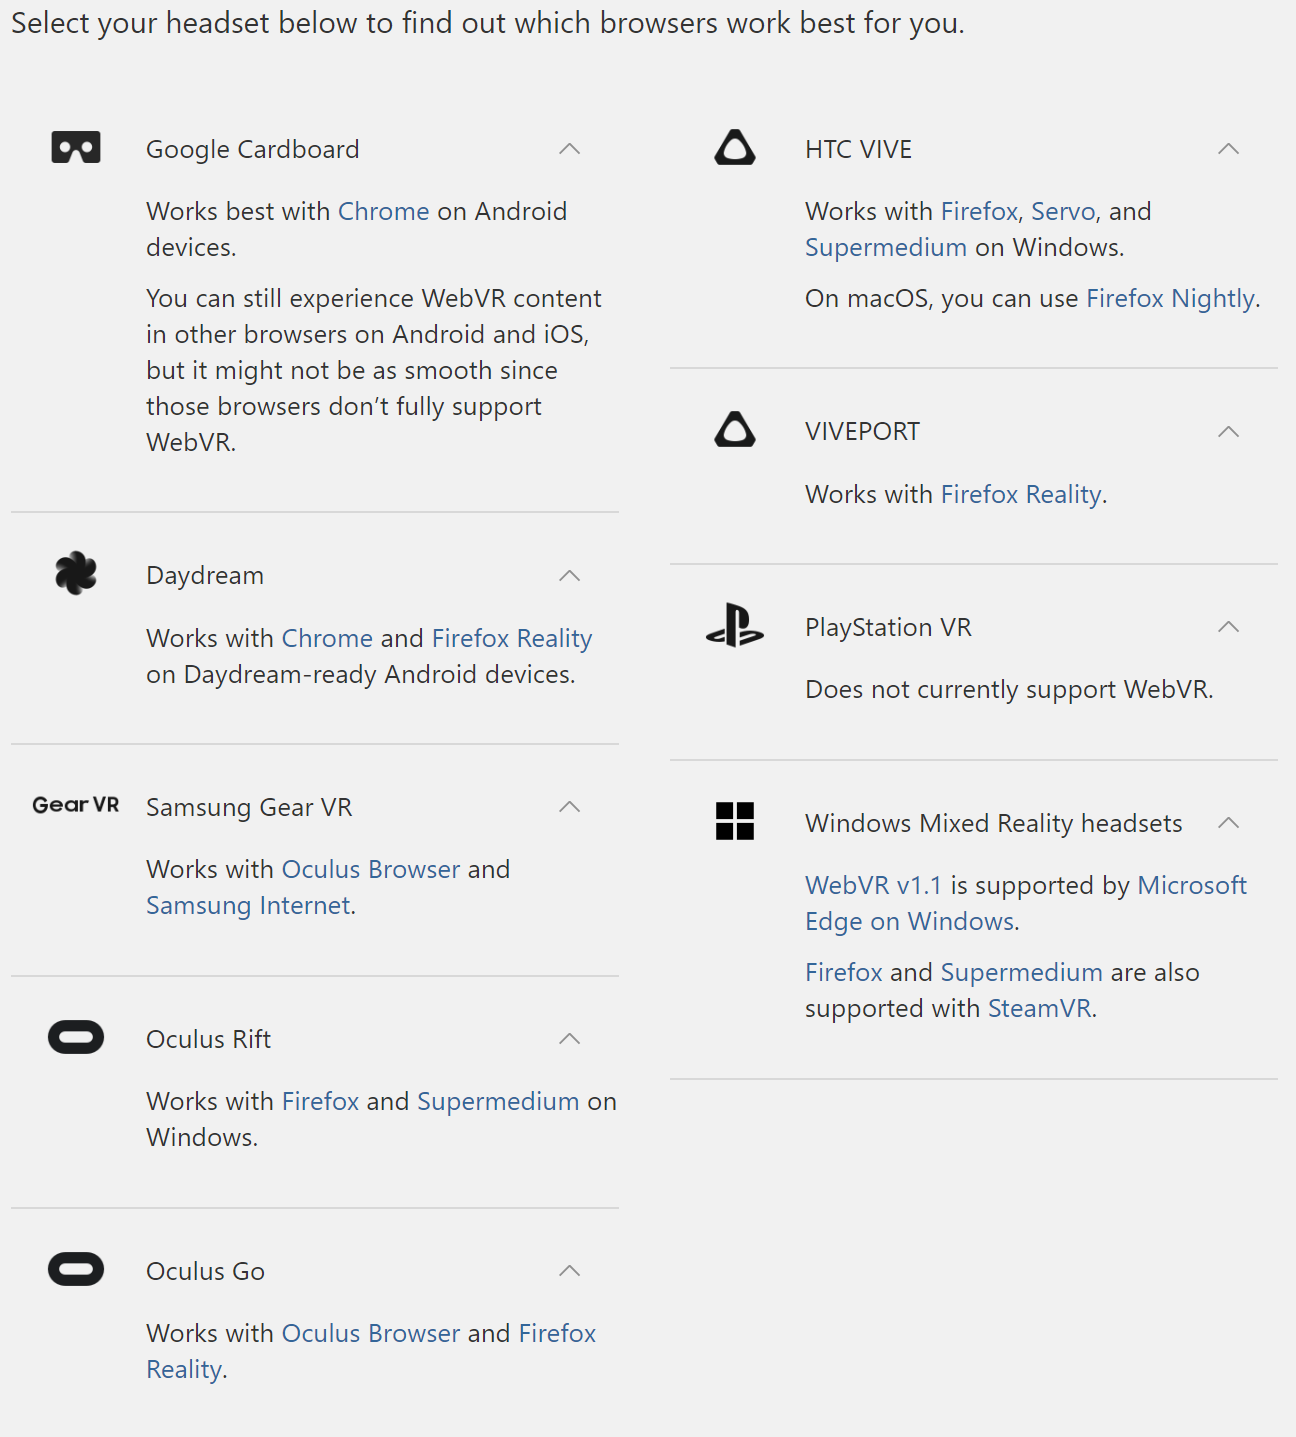
\includegraphics[width=\textwidth]{images/supportedBrowsers.png}
 
  \subsubsection{Entwicklung}
 Die Grundtechnik von WebVR ist WebGL, die auf OpenGL basiert. OpenGL ist eine Application Programming Interface (API), um 2D und 3D Grafik darzustellen. \glqq WebGL is a cross-platform, royalty-free web standard for a low-level 3D graphics API based on OpenGL ES, exposed to ECMAScript via the HTML5 Canvas element. \grqq \citep{23} Das heißt, dass die Grafiken durch WebGL als ein Form umwandelt, der von Browser verstehen kann. 
 
 Die Programmierung direkt mit WebGL ist kompliziert und zeitaufwendig. Um effizienter zu entwickeln werden erfahrungsmäßig Javascript 3D Engines benutzt, z.B. three.js, PlayCanvas und Unity.
 
 Die three.js ist eine open source JavaScript Bibiliothek, die die WebGL Objekten einpackt. Durch den Funktionen von three.js Objekten können die WebGL Objekten manipuliert werden. Die Funktionsweise ist änhlich wie JQuery zu JavaScript. Auf three.js werden unterschiedliche Frameworks beispielsweise A-Frame, React 360 und Vizor entwickelt.
 
 PlayCanvas ist eine web-basierte visuelle Entwicklungsplattform für interaktive Inhalte auf Web. Die Entwicklung wird in Browser durchgeführt.
 
 Mit Unity WebVR Assets von Mozilla kann das Unity Projekt als WebVR gebildet werden.

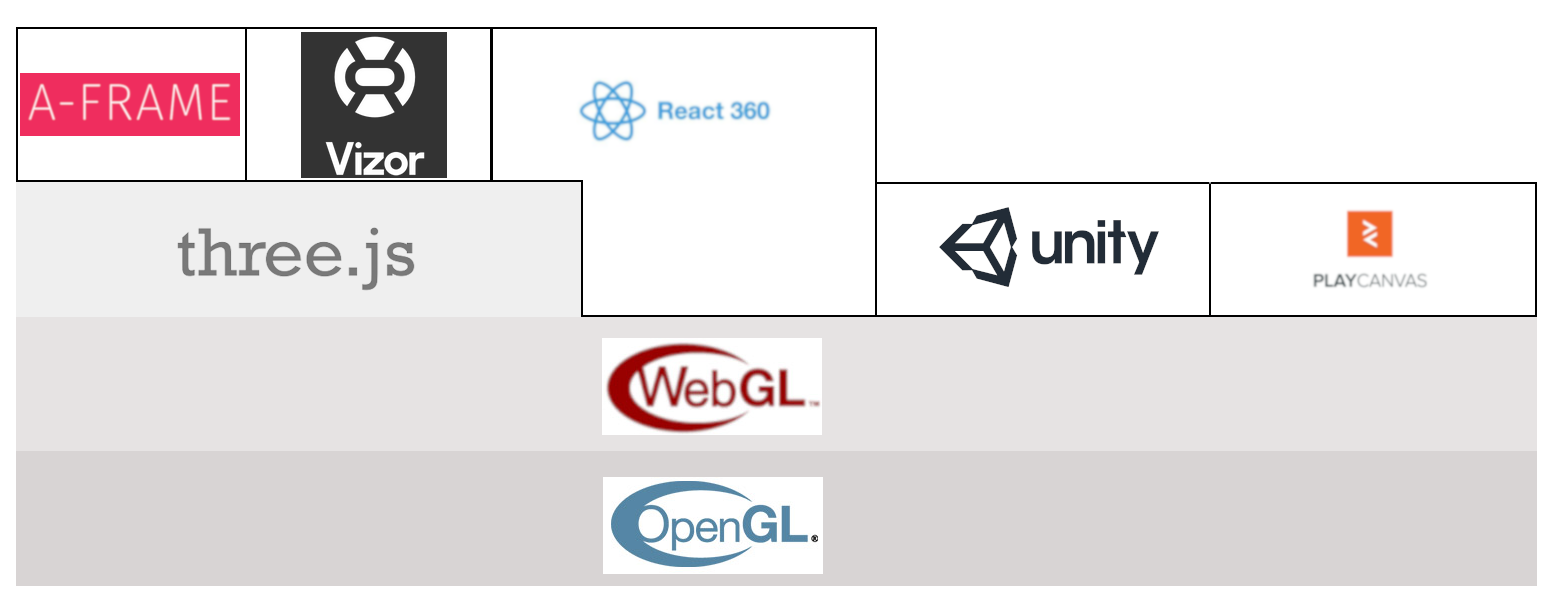
\includegraphics[width=\textwidth]{images/webVRStruckture.png}

\section{Zusammenfassung}
E-Learning gilt schon als eine wichtige Werkzeug im Bereich Ausbildung. Obwohl Viele Unternehmen beispieweise Walmart\citep{24} haben schon von VR-Training profitiert, ist VR-Training noch nicht so weit verbreitet. Allerdings wird VR-Training eine unersetzbare Rolle auf dem Markt für Schulung spielen, wenn die VR Geräte günstiger und benutzerfreundlicher sind.

Danke für die Entwicklung von WebVR ist es möglich, E-Learning und VR-Training zu verbinden. Damit können die beide sich gegenseitig ergänzen.


